\documentclass[tikz,border=10pt]{standalone}
% No extra TikZ libraries needed
\begin{document}
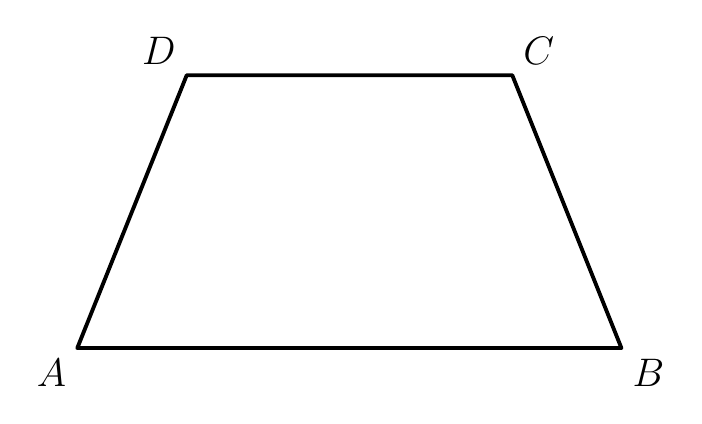
\begin{tikzpicture}[line join=round, line width=1.4pt]
  % Vertices: s = 0.017582 cm/px, centred on ink bbox (cx=265.5, cy=144.5), y flipped
  \coordinate (A) at (-3.4832,-1.7318);
  \coordinate (B) at (3.4268,-1.7318);
  \coordinate (C) at (2.0414,1.7318);
  \coordinate (D) at (-2.0940,1.7318);
  % Edges AB, BC, CD, DA
  \draw (A) -- (B) -- (C) -- (D) -- cycle;
  % Labels just outside each vertex
  \node[below left,  font=\fontsize{14.5}{17.4}\selectfont] at (A) {$A$};
  \node[below right, font=\fontsize{14.5}{17.4}\selectfont] at (B) {$B$};
  \node[above right, font=\fontsize{14.5}{17.4}\selectfont] at (C) {$C$};
  \node[above left,  font=\fontsize{14.5}{17.4}\selectfont] at (D) {$D$};
\end{tikzpicture}
\end{document}